\chapter{Neural Networks}

\section{Introduzione}
\`E stato visto come il perceptron pu\`o imparare un modello lineare utilizzando la funzione attivatrice e il peso degli input.
Funzioni attivatrici tradizionali sono non lineari come la sigmoide $h(x) = \frac{1}{1+e^{-x}}$ e la tangente iperbolica $h(x) = \frac{e^x-e^{-x}}{e^x+e^{-x}}$, mentre funzioni attivatrici pi\`u moderne sono la rectified linear unit \emph{ReLU}: $h(x) = \max(0,x)$ e la Leaky ReLU $h(x) = \max(\alpha x,x)$ con $\alpha$ costante piccola.

\subsection{Perceptron}
Il perceptron si pu\`o considerare come un neurone artificiale, una funzione non lineare parametrizzata con un range di output ristretto:
$$\hat{y} = h\bigl(\sum\limits_i\theta_ix_i\bigr) = h(\theta^Tx)$$

\subsubsection{Rosemblatt}
Nel $1958$ Rosemblatt considera il perceptron \ref{fig:chapter11-00} come una macchina per la classificazione lineare: si imparano i pesi e si considera il bias: un peso per input, si moltiplicano i pesi con gli input rispettivi e si aggiunge il bias.
Se il risultato \`e pi\`u grande di una threshold si ritorna $1$, altrimenti $0$.

\begin{figure}
	\centering
	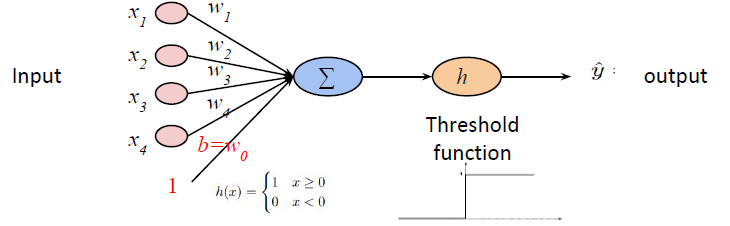
\includegraphics[width=0.6\linewidth]{imgs/chapter11/img0}
	\caption{Perceptron}
	\label{fig:chapter11-00}
\end{figure}

	\subsection{Multi layer perceptron}
	Il perceptron presenta diverse limitazioni: non \`e in grado di risolvere problemi non linearmente separabili come quello dello \emph{XOR}. 
	Per capire cosa intendiamo quando diciamo che \emph{XOR} non \`e un problema linearmente separabile guarda la figura \ref{fig:chapter11-01}.
	Per superare questo problema Minsky e Papert nel $1969$ sviluppano il multi-layer perceptron \emph{MLP}.
	Questi sono neuroni artificiali densamente connessi che realizzano composizioni di funzioni non lineari utilizzati per la classificazione e regressioni.
	Sono composti da un input layer, diversi hidden layer e un output layer.
	L'informazione viene propagata dall'input all'output senza cicli: l'\emph{MLP} \`e un directed acyclic graph \emph{DAG}.
	La computazione viene svolta dalla composizione di un numero di funzioni algebriche implementate dalle connessioni, pesi e biases dei layer di output e nascosti.
	Gli hidden layer computano delle rappresentazioni intermedie.

		\subsubsection{Single layer neural network}
		In una single layer neural network il primo layer $(1)$ riceve i dati dall'input e li passa a un layer nascosto $(2)$, che a sua volta li passa all'output \ref{fig:chapter11-02}: $\hat{y}_k$:
		\begin{itemize}
			\item[$(1)$] $z_j = \sum\limits_i\theta^{(1)}_{i,j}x_i + \theta_{0,j}^{(1)}$.
			\item[$(2)$] $\hat{y}_k = h\bigl(\sum\limits_i\theta^{(2)}_{i,j}h(z_i)+\theta^{(2)}_{0,j}i\bigr)$.
		\end{itemize}
		\begin{figure}
			\centering
			\begin{minipage}{.5\textwidth}
				\centering
				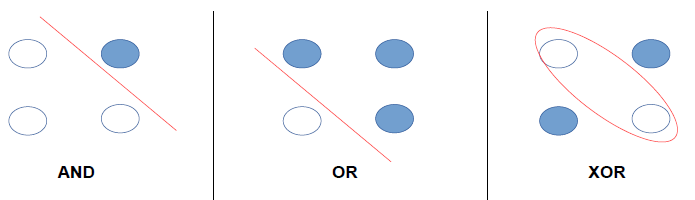
\includegraphics[width=1\linewidth]{imgs/chapter11/img1}
				\caption{Problemi linearmente e non linearmente separabili}
				\label{fig:chapter11-01}
			\end{minipage}%
			\begin{minipage}{.5\textwidth}
				\centering
				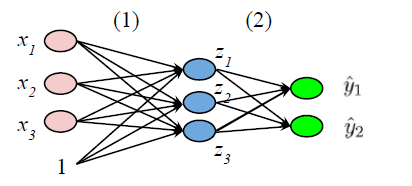
\includegraphics[width=0.7\linewidth]{imgs/chapter11/img2}
				\caption{Feed-forward Neural Networks}
				\label{fig:chapter11-02}
			\end{minipage}
		\end{figure}


	\subsection{First AI winter}
	Il first AI winter nasce in quanto si rende difficile fare del training su un \emph{MLP}: non ci si pu\`o applicare la regola del perceptron in quanto si aspetta di conoscere il target desiderato.
	Per gli hidden layer infatti \`e impossibile conoscere il target desiderato.

		\subsubsection{Backpropagation}
		Il problema del training del \emph{MLP} viene risolto attraverso la backpropagation nel $1986$, che permette pertanto il learning di \emph{MLP} per funzioni complicate.
		Algoritmi efficienti permettono di processare grandi training sets e permettono architetture complesse di neural networks.
		Tutt'oggi si trova al nucleo del training delle reti neurali.
		Il training pertanto consiste di tre passaggi \ref{fig:chapter11-03}:
		\begin{multicols}{2}
			\begin{itemize}
				\item Forward propagation: si sommano gli input, si produce attivazione e si fa feed-forward.
				\item Si stima l'errore.
				\item Si propaga all'indietro il segnale di errore e lo si usa per aggiornare i pesi.
			\end{itemize}
		\end{multicols}
		
		\begin{figure}
			\centering
			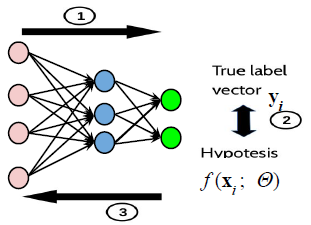
\includegraphics[width=0.4\linewidth]{imgs/chapter11/img3}
			\caption{Backpropagation}
			\label{fig:chapter11-03}
		\end{figure}
		
		Il learning diventa un problema di ottimizzazione, in cui dati i training samples $T=\{(x_1,y_1),\dots,(x_N,y_N)\}$ si devono aggiustare tutti i pesi della rete $\Theta$ in modo che una funzione di costo sia minimizzata:
		$$\min_\Theta\sum\limits_i L(y_i, f(x_i,\Theta))$$
		Si deve pertanto scegliere la loss function, aggiornare i pesi di ogni layer con il gradient descent e usare la backpropagation del segnale di errore per computare il gradiente efficientemente.
		
		\subsubsection{CNN e LSTM}
		La backpropagation permette importanti sviluppi nel campo come le convolutional neural networks e le recurrent long-short term memory networks negli anni $90$.

	\subsection{Second AI winter}
	Si nota come queste reti neurali non possono sfruttare molti layer a causa di overfitting e del vanishing gradient: la moltiplicazione di piccoli numeri nel training causa a questi di diventare sempre pi\`u piccoli fino a renderli non significativi, gli aggiornamenti dei pesi nei primi livelli sono molto meno significativi di quelli negli ultimi.
	Inoltre non si disponeva della capacit\`a computazionale necessaria e mancavano grandi dataset annotati.

		\subsubsection{SVM e metodi di kernel}
		A causa di questi problemi diventano popolari le Kernel machines come gli SVM in quanto riuscivano ad ottenere accuratezze simili alle reti neurali, possedevano meno euristiche e iperparametri e una prova di generalizzazione.

	\subsection{Deep learning revolution}
	Nel $2006$ si utilizza un nuovo modo per inizializzare i pesi: ogni layer viene trainato singolarmente attraverso unupervised training come contrastive divergence e i pesi si sistemano con un round di supervised learning.
	Nasce cos\`i alexnet, una rete CNN simile a LeNet ma trainata con due GPU e con migliorie tecniche come ReLU, dropout e data augmentation.
	
	\subsection{Caratteristiche del deep learning}
	Si nota come il deep learning, a differenza del machine learning tradizionale non richiede la creazione di feature a tavolino: la loro estrazione avviene infatti negli hidden layers.
	Si nota pertanto come una rete neurale \`e una composizione di moduli, funzioni connesse gerarchicamente con parametri $\Theta$.

\section{Feedforward networks}
Nelle reti feed forward la funzione $f$ \`e la composizione di multiple funzioni:
$$f(x) = f^{(n)}(\dots(f^{(1)}(x)\dots)$$
L'obiettivo \`e quello di approssimare una funzione sconosciuta ideale $f^*:\mathcal{X}\rightarrow\mathcal{Y}$, in cui il modello ideale \`e $y = f^*(x)$.
Per queste reti si definisce una mappatura parametrica $y = f(x,\theta)$ e si imparano i parametri per trovare una buona approssimazione di $f^*$ dai sample disponibili.
L'informazione fluisce dall'input, verso computazioni intermedie e si produce l'ouput.
La composizione delle funzioni pu\`o essere descritta come un \emph{DAG}, in cui la profondit\`a \`e il massimo $i$ nella catena di composizione delle funzioni.
Il layer finale viene chiamato layer di output. 
La rete neurale in figura \ref{fig:chapter11-04} ha una profondit\`a di 3.
\begin{figure}
	\centering
	\begin{minipage}{.5\textwidth}
		\centering
		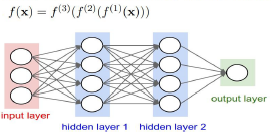
\includegraphics[width=0.8\linewidth]{imgs/chapter11/img4}
		\caption{}
		\label{fig:chapter11-04}
	\end{minipage}%
	\begin{minipage}{.5\textwidth}
		\centering
		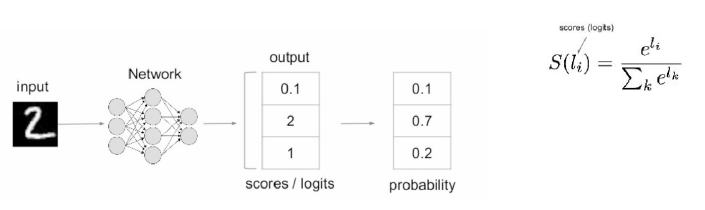
\includegraphics[width=1\linewidth]{imgs/chapter11/img5}
		\caption{Funzione di costo}
		\label{fig:chapter11-05}
	\end{minipage}
\end{figure}



	\subsection{Training}
	Per il training si deve ottimizzare $\theta$ per portare $f(x,\theta)$ il pi\`u vicino possibile a $f^*(x)$.
	Questa viene valutata a diverse istanze di $x$ di training data, che specifica solamente l'output dei layer finali.
	L'output dei layer intermedi non viene specificato, da cui il nome hidden layers.
	Questo \`e simile a progettare una macchina basata su gradient descent: il problema diventa non convesso e non c'\`e garanzia di convergenza. Ci sono molti minimi locali, e molto probabilmente finiremo in un minimo locale in fase di training. 
	Per questo \`e importante inizializzare i pesi di una NN con valori random, piccoli e uniformemente distribuiti e per esempio fare training di 10 NN diverse e vedere quale \`e la migliore sul training set.
	In particolare per applicare il gradient descent si deve specificare un modello, una funzione di costo e la rappresentazione dell'output.
	
	\subsection{Scelte di modellamento}
	Per modellare una feedforward network si devono scegliere:
	\begin{multicols}{2}
		\begin{itemize}
			\item Funzione di costo.
			\item Forma dell'output.
			\item Funzione di attivazione.
			\item Architettura.
			\item Ottimizzatore.
		\end{itemize}
	\end{multicols}

		\subsubsection{Funzione di costo}
		La funzione di costo dice quanto la rete si comporta bene rispetto ai training data:
		$$\mathcal{L}(w) = distance(f_\theta(x), y)$$
		Calcola ovvero la discrepanza tra la predizione e la label effettiva,
		Si possono applicare loss gi\`a viste e tipicamente si converte l'output in probabilit\`a come attraverso softmax. 
		Alcune funzioni di costo si adattano bene a problemi di classificazione altre a problemi di regression \ref{fig:chapter11-05}.

\paragraph{Cross-entropy}
La cross-entropy loss \`e la loss function pi\`u comune applicata con softmax \ref{fig:chapter11-06}:
$$\mathcal{L}_i = -\sum\limits_ky_y\log(S(l_k)) = -\log(S(l))$$

\begin{figure}
	\centering
	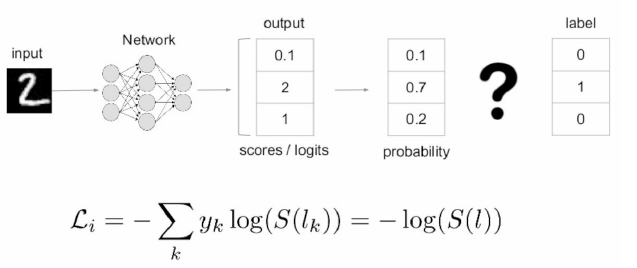
\includegraphics[width=0.6\linewidth]{imgs/chapter11/img6}
	\caption{Cost function: Cross-Entropy}
	\label{fig:chapter11-06}
\end{figure}

		\subsubsection{Output layers}
		Si nota come la scelta della loss function sia correlata alla scelta dell'unit\`a di output.

		\paragraph{Linear}
		Data una feature $h$ un unit\`a di un layer di output lineari d\`a:
		$$\hat{y} = W^Th+b$$
		Questi unit\`a non si saturano (mantiene il gradiente lontano da $0$), offrono poca difficolt\`a agli algoritmi basati sull'ottimizzazione del gradiente.
		Si nota come un output del modello vicino a $0$ \`e problematico.
		Utilizzata spesso nei problemi di regressione.
		
		\paragraph{Softmax}
		Softmax permette di produrre probabilit\`a normalizzate nell'output layer, pertanto produce:
		$$S(l_i) = \frac{e^{l_i}}{\sum\limits_ke^{l_k}}$$
		Utilizzata spesso in problemi di classificazione.
		\subsubsection{Hidden units}
		All'interno di una hidden unit si accetta un input $x$, si computa una trasformazione affine: $z = w^Tx+b$, si applica element-wise una funzione non lineare $h(z)$ e si ottiene l'output $h(z)$.
		La scelta da compiere si basa su quale $h$ (funzione di attivazione) utilizzare.

		\paragraph{Rectified linear units (RELU)}
		Una RELU presenta un gradiente di $0$ o $1$, facile da ottimizzare simile alle unit\`a linari.
		D\`a gradienti grandi e consistenti quando attiva, ma non \`e sempre differenziabile, risolvibile attraverso una derivata da un lato a $z=0$.
		Ne esistono diverse varianti che risolvono il problema che l'unit\`a muore quando il gradiente \`e $0$ \ref{fig:chapter11-07}:
		\begin{multicols}{2}
			\begin{itemize}
				\item ReLu: $y_i = 0$ per $x < 0$ o $y_i = x_i$ per $x >0$.
				\item Leaky Relu: $y_i = a_ix_i$ per $x < 0$ o $y_i = x_i$ per $x >0$.
				\item Randomized Leaky Relu: $y_{ji} = a_{ji}x_{ji}$ per $x < 0$ o $y_{ji} = x_{j}i$ per $x >0$.
			\end{itemize}
		\end{multicols}
		\begin{figure}
			\centering
			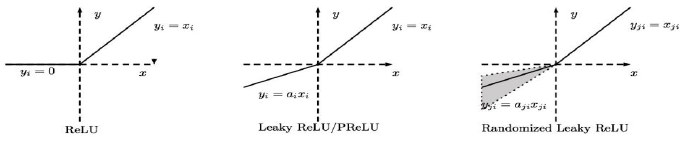
\includegraphics[width=0.8\linewidth]{imgs/chapter11/img7}
			\caption{Funzione di costo}
			\label{fig:chapter11-07}
		\end{figure}
		
		\paragraph{Sigmoid e Tanh}
		Questi due tipi di hidden unit riducono il tipo di non linearit\`a restringendo l'output ai range $[0,1]$ e $[-1,1]$.
		Si saturano lungo la maggior parte del dominio e sono fortemente sensibili unicamente quando l'input \`e pi\`u vicino a $0$ \ref{fig:chapter11-08}.
		La saturazione rende l'apprendimento basato sul gradient pi\`u difficile.
		\begin{multicols}{2}
			\begin{itemize}
				\item Sigmoide: $h(x) = \frac{1}{1+e^{-x}}$.
				\item Tangente iperbolica: $h(x) = \frac{e^x-e^{-x}}{e^x+e^{-x}}$.
			\end{itemize}
		\end{multicols}
		\begin{figure}
			\centering
			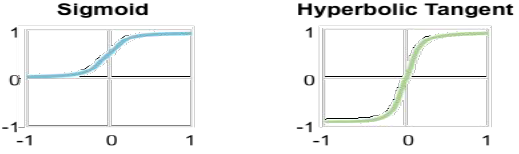
\includegraphics[width=0.6\linewidth]{imgs/chapter11/img8}
			\caption{Sigmoid e Tanh}
			\label{fig:chapter11-08}
		\end{figure}

		\subsubsection{Architettura}
		La decisione rispetto alla profondit\`a e larghezza di una rete neurale si basa principalmente su risultati empirici.
		Un risultato teorico da parte di Cybenko $1989$: reti a $2$-layer con output lineari con del squashing non-linearity nelle hidden-unit possono approssimare ogni funzione continua su dominio compatto ad accuratezza arbitraria.
		Questo risultato \`e valido anche per funzioni non lineari.
		Questo implica che per ogni funzione che si cerca di imparare, un grande \emph{MLP} \`e in grado di impararla.
		Nonostante questo non \`e garantito che l'algoritmo di training sia capace di imparare tale funzione (per problemi legati all'overfitting, o di ottimizzazione).

	\subsection{Backpropagation}
	La backpropagation \`e il modo in cui la rete impara i propri pesi.
	Consiste di tre passaggi:
	\begin{multicols}{2}
		\begin{enumerate}
			\item Feedforward propagation: si accetta l'input $x$, si passa attraverso stages intermedi e si ottiene l'output.
			\item Si usa l'output computato per computare un costo scalare dipendente dalla loss function.
			\item La backpropagation permette all'informazione di fluire all'indietro dal costo per computare il gradiente.
		\end{enumerate}
	\end{multicols}
	Si utilizza il gradient descent: si necessitano le derivate degli errori per ogni peso nella rete:
	$$w^{(i)}_{jk} := w^{(i)}_{jk} - \eta\frac{\partial L}{\partial w^{(i)}_{jk}}$$
	Dai training data non si conosce cosa dovrebbero fare gli hidden layers, ma si pu\`o computare quanto velocemente l'errore cambia cambiando la loro attivit\`a: si usano le derivate dell'errore con rispetto alle sue attivit\`a.
	Ogni hidden unit pu\`o avere effetto su diverse unit\`a di output e effetti separati sull'errore che vengono combinati.
	Si pu\`o calcolare la derivata di queste unit\`a efficentemente: una volta che si ha la derivata delle attivit\`a nascoste \`e facile ottenere l'errore per i pesi che arrivano.

		\subsubsection{Operazione di feedforward}
		Dall'input all'output \ref{fig:chapter11-09}:
		$$\hat{y}(x;w) = f\bigl(\sum\limits_{i=1}^mw_j^{(l)}h\bigl(\cdots h\bigl(\sum\limits_{i = 1}^dw_{ij}^{(1)}x_i + w_{0j}^{(1)}\bigr)\cdots\bigr) + w_0^{(l)}\bigr)$$
		
		\begin{figure}
			\centering
			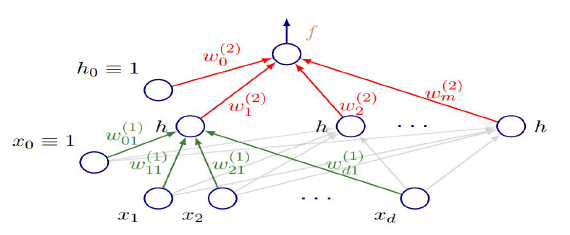
\includegraphics[width=0.6\linewidth]{imgs/chapter11/img9}
			\caption{Operazione di feedforward}
			\label{fig:chapter11-09}
		\end{figure}
		
		\subsubsection{Computare l'errore e train}
		L'errore della rete sul training set:
		$$L(X;w) = \sum\limits_{i=1}^N\frac{1}{2}(y_i-\hat{y}(x_i;w))^2$$
		Non ha una soluzione di forma causa, si utilizza il gradient descent. 
		Nota come stiamo utilizzando l'errore quadratico, e non c'\`e un regolarizzatore, che utilizzavamo per ridurre il problema dell'overfitting. 
		Nelle NN il problema dell'overfitting si risolve facendo early stopping, ossia fermiamo il training prima di andare in overfitting.
		Si deve calcolare la derivata di $L$ su un singolo esempio.
		Si pu\`o considerare un modello lineare semplice con output $\hat{y} = \sum\limits_jw_jx_{ij}$:
		$$\frac{\partial L(X_i)}{\partial w_j} = (\hat{y}_i -y_i)x_{ij}$$
		
		\subsubsection{Backpropagation}
		L'unit\`a di attivazione generale in una rete multilayer:
		$$z_t = h\bigl(\sum\limits_jw_{jt}z_j\bigr)$$
		La forward propagation calcola per ogni unit\`a $a_t = \sum\limits_j w_{jt}z_j$.
		Dove $a_t$ \`e l'input della funzione di attivazione di un'unit\`a di livello $t$.
		Ora
		$$\frac{\partial L}{\partial w_{jt}} = \frac{\partial L}{\partial a_t}z_j$$
		Sia $\partial a_t = \delta_t$ e l'unit\`a di output con attivazione lineare $\delta_t = \hat{y} -t$.
		L'unit\`a hidden $t$ che manda l'output all'unit\`a $S$:
		\begin{align*}
			\delta_t &= \sum\limits_{s\in S} = \sum\limits_{s\in S}\frac{\partial L}{\partial a_s}\frac{\partial a_s}{\partial a_t}=\\
			&= h'(a_t)\sum\limits_{s\in s} w_{ts}\delta_s
		\end{align*}
		
		\subsubsection{Esempio}
		Sia l'output $f(a) = a$ e l'hidden: $h(a) = tanh(a) = \frac{e^a-e^{-a}}{e^a+e^{-a}}$, ora $h'(a) = 1-h(a)^2$.
		Dato $x$, il feedforward inputs:
		\begin{multicols}{2}
			\begin{itemize}
				\item Input to hidden $a_j = \sum\limits_{i = 0}^d w_{ij}^{(1)}x_i$, con il bias rimosso per semplicit\`a.
				\item Hidden input $z_j = tanh(a_j)$.
				\item Net output $\hat{y} = a = \sum\limits_{i = 0}^m w_j^{(2)} z_j$.
			\end{itemize}
		\end{multicols}
		Guarda la figura \ref{fig:chapter11-14} per una rappresentazione grafica.
		L'errore sull'esempio $x$ \`e $L= \frac{1}{2}(y-\hat{y})^2$ e l'unit\`a di output: $\delta = \frac{\partial L}{\partial a} = y - \hat{y}$.
		Si computa $\delta$ per le unit\`a hidden:
		$$\delta_j = (1-z_y)^2w_j^{(2)}\delta$$
		Le derivate con rispetto ai pesi:
		\begin{multicols}{2}
			\begin{itemize}
				\item $\frac{\partial L}{\partial w_{ij}^{(1)}} = \delta_jx_i$.
				\item $\frac{\partial L}{\partial w_j^{(2)}} = \delta z_j$.
			\end{itemize}
		\end{multicols}
		E si aggiornano i pesi:
		\begin{multicols}{2}
			\begin{itemize}
				\item $w_j = w_j - \nu \delta z_j$.
				\item $w_{ij}^{(1)} = w_{ij}^{(1)} - \nu \delta_jx_i$.
			\end{itemize}
		\end{multicols}
		\begin{figure}
			\centering
			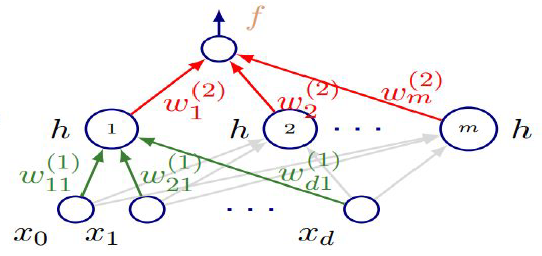
\includegraphics[width=0.6\linewidth]{imgs/chapter11/img14}
			\caption{La rete}
			\label{fig:chapter11-14}
		\end{figure}
		
		\paragraph{Output multidimensionale}
		Per l'output multidmensionale la loss sull'esempio \`e:
		$$\frac{1}{2}\sum\limits_{k = 1}^K(y_k-\hat{y}_k)^2$$
		Per ogni unit\`a di output: $\delta_k = y_k - \hat{y}_k$.
		Per l'unit\`a hidden $j$:
		$$\delta_j = (1-z_j)^2\sum\limits_{k=1}^Lw_{jk}^{(2)}\delta_k$$

	\subsection{Scelta di un ottimizzatore}
	Il gradient \`e il vettore delle derivate parziali con rispetto di tutte le coordinate dei pesi:
	$$\nabla_w L = \bigl[\frac{\partial L}{\partial w_1}, \cdots, \frac{\partial L}{\partial w_N}\bigr]$$
	Ogni derivata parziale misura quanto velocemente la loss cambia in una direzione.
	Quando il gradiente \`e zero, la loss non cambia in nessuna direzione.
	D\`a problemi nei saddle points e nei local minima.
	Il gradient descent trova pertanto l'insieme di parametri che rendono la loss il pi\`u piccola possibile.
	I cambi nei parametri dipendono dal gradiente della loss con rispetto dei pesi della rete.
	La backpropagation \`e il metodo per computare i gradienti.
	Si analizzano altri miglioramenti come Stochastic gradient descent.
	Il gradient descent nelle reti neurali pu\`o essere calcolato in diversi modi.

		\subsubsection{Batch Gradient Descent (BGD)}
		In BGD i gradienti sono computati su ogni update per l'intero training con un alto costo computazionale ma garantendo una grande stabilit\`a nella stima del gradiente.
		Il learning rate $\varepsilon_k$ pu\`o cambiare linermente nel tempo \ref{fig:chapter11-10}.\\
		\begin{algorithm}[H]
\DontPrintSemicolon
\SetKwComment{comment}{$\%$}{}
\SetKw{Int}{int}
\SetKw{To}{to}
\SetKw{IsNot}{is not}
\SetKw{Not}{not}
\SetKw{Return}{return}
\SetKw{Require}{return}
\SetKwData{Item}{item}
\SetKwFunction{Min}{min}
\SetKwFunction{GradientDescent}{Batch Gradient Descent at iteration K}

\caption{\protect\GradientDescent}
	\Require : Learning rate $\varepsilon_k$\;
	\Require : Initial Parameter $\theta$\;
	\While{stopping criteria not met}{
		\comment{Compute gradient estimate over $N$ examples}
		g = $+\frac{1}{N}\nabla_\theta\sum_i L(f(x^{(i)};\theta),y^{(i)}$\;
		\comment{Apply update}
		$\theta = \theta -\varepsilon_k g$\;
	}
\end{algorithm}

		
		\begin{figure}
			\centering
			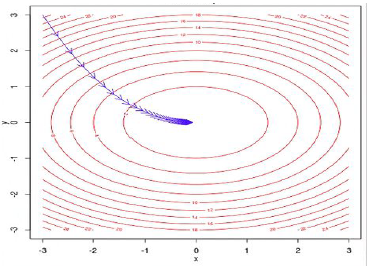
\includegraphics[width=0.6\linewidth]{imgs/chapter11/img10}
			\caption{Batch Gradient Descent (BGD)}
			\label{fig:chapter11-10}
		\end{figure}
		
		\subsubsection{Stochastic gradient descent (SGD)}
		In SDG si computa il gradiente solo su un campione scelto casualmente e non sull'intero training set in modo da ottenere performance migliori.
		Il learning rate cambia ad ogni passo, tipicamente decade linearmente \ref{fig:chapter11-11}.
		
		
\begin{algorithm}
\DontPrintSemicolon
\SetKwComment{comment}{$\%$}{}
\SetKw{Int}{int}
\SetKw{To}{to}
\SetKw{IsNot}{is not}
\SetKw{Not}{not}
\SetKw{Return}{return}
\SetKw{Require}{return}
\SetKwData{Item}{item}
\SetKwFunction{Min}{min}
\SetKwFunction{GradientDescent}{Stochastic Gradient Descent at iteration K}

\caption{\protect\GradientDescent}
	\Require : Learning rate $\varepsilon_k$\;
	\Require : Initial Parameter $\theta$\;
	\While{stopping criteria not met}{
		\comment{Compute gradient estimate over sample example ($x^{(i)}, y^{(i)}$) from training set}
		g = $+\nabla_\theta\sum_i L(f(x^{(i)};\theta),y^{(i)}$\;
		\comment{Apply update}
		$\theta = \theta -\varepsilon_k g$\;
	}
\end{algorithm}

		
		\begin{figure}
			\centering
			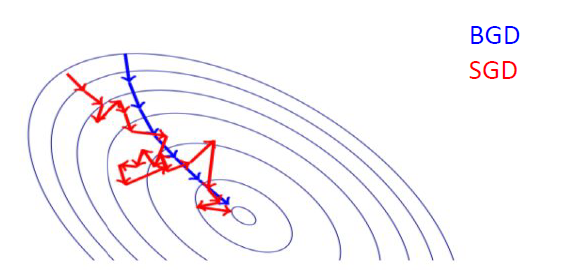
\includegraphics[width=0.6\linewidth]{imgs/chapter11/img11}
			\caption{BGD vs SGD}
			\label{fig:chapter11-11}
		\end{figure}
		
		\subsubsection{Mini-batch gradient descent}
		Le minibatches risolvono il problema di SDG rispetto ai dati rumorosi.
		Il tempo di computazione per aggiornamento non dipende dal numero di esempi di training $N$, permettendo la creazione di minibatches pi\`u grandi che vengono computate parallelamente.
		Sono tipicamente di dimensione $2^n$ per le propriet\`a di calcolo della GPU.
		
		\subsubsection{Momento}
		Un problema di BGD e SGD \`e il fatto che minimizzano l'errore in molto tempo.
		Una soluzione diversa \`e data dalla tecnica del momento, che introduce un vettore velocit\`a $v$ di aggiornamenti, una media con decay esponenziale per i gradienti utilizzato per aggiornare i pesi.
		Introduce un vettore momento che regola il trade-off tra il gradiente allo step corrente e quelle vecchie. 
		In particolare si utilizza una media mobile pesata dei gradienti passati, in cui i gradienti nel passato recente hanno pi\`u importanza di quelli nel passato lontano che sommata al gradiente calcolato in un punto aiuta a superare i punti sella, dove altrimenti il gradiente sarebbe zero e la fase di training si allungherebbe notevolmente, o si fermerebbe. \\
		\begin{algorithm}
\DontPrintSemicolon
\SetKwComment{comment}{$\%$}{}
\SetKw{Int}{int}
\SetKw{To}{to}
\SetKw{IsNot}{is not}
\SetKw{Not}{not}
\SetKw{Return}{return}
\SetKw{Require}{return}
\SetKwData{Item}{item}
\SetKwFunction{Min}{min}
\SetKwFunction{GradientDescent}{Stochastic Gradient Descent with momentum}

\caption{\protect\GradientDescent}
	\Require : Learning rate $\varepsilon_k$\;
	\Require : Momentum parameter $\alpha$\;
	\Require : Initial Parameter $\theta$\;
	\Require : Initial velocity $v$\;
	\While{stopping criteria not met}{
		\comment{Compute gradient estimate over sample example ($x^{(i)}, y^{(i)}$) from training set}
		g = $+\nabla_\theta\sum_i L(f(x^{(i)};\theta),y^{(i)}$\;
		\comment{Compute velocity update}
		$v = \alpha v - \varepsilon_k g$\;
		\comment{Apply update}
		$\theta = \theta -\varepsilon_k g$\;
	}
\end{algorithm}

		
		\subsubsection{Adaptive learning rate method}
		Alcune volte \`e bene usare un learning rate diverso per ogni peso.
		Un metodo che lo implementa \`e Adagrad o adaptive gradient optimizer.
		Questo fa downscale di un parametro del modello della radice della somma dei quadrati dei valori storici, in questo modo parametri con una grande derivata parziale hanno learning rate che si abbassano rapidamente.
		Si adatta al learning rate dei parametri svolgendo aggiornamenti minori associati con feature che pi\`u frequenti e grandi per feature meno frequenti.
		Utile per gestire dati sparsi.\\
		\begin{algorithm}[H]
\DontPrintSemicolon
\SetKwComment{comment}{$\%$}{}
\SetKw{Int}{int}
\SetKw{To}{to}
\SetKw{IsNot}{is not}
\SetKw{Not}{not}
\SetKw{Return}{return}
\SetKw{Require}{return}
\SetKwData{Item}{item}
\SetKwFunction{Min}{min}
\SetKwFunction{GradientDescent}{AdaGrad}

\caption{\protect\GradientDescent}
	\Require : Learning rate $\varepsilon_k$\;
	\Require : Initial Parameter $\theta,\delta$\;
	r = 0\;
	\While{stopping criteria not met}{
		\comment{Compute gradient estimate over sample example ($x^{(i)}, y^{(i)}$) from training set}
		$\hat{g} = +\nabla_\theta\sum_i L(f(x^{(i)};\theta),y^{(i)})$\;
		\comment{Compute velocity update}
		r = r + $f\circ \hat{g}$
		\comment{Compute update}
		$\Delta\theta = -\frac{\varepsilon_k}{\delta+\sqrt{r}}\circ i\hat{g}$\;
		$\theta = \theta +\Delta\theta$\;
	}
\end{algorithm}


\section{Convolutional Neural Netwoks (CNN)}
Le convolutional neural networks sono un tipo di feedforward neural networks.
Queste gestiscono molto bene uno spazio di input localmente strutturato, spazialmente o temporalmente.
Sono inoltre molto utili quando l'obiettivo non \`e la classificazione: ottengono grandi risultati in region extraction, feature detection, semantic segmentation e structured regression.
In particolare le CNN imparano una gerarchia di features: ognuno dei layer estrae delle features dall'output del layer precedente.
Tutti i layer vengono trainati insieme.
Si definiscono CNN le reti che usano la convolution al posto di una moltiplicazione tra matrici generica in almeno uno dei loro livelli.
Si definisce convolution:
$$S(i, j) = (I\cdot K)(i,j) = \sum\limits_M\sum\limits_NI(m,n(K(i-m,j-n)$$

	\subsection{Origini}
	Questo tipo di reti \`e stato ispirato dalla corteccia visiva dei mammiferi: questa contiene un ordinamento di cellule sensibili a piccole sotto regioni del campo visivo, dette campo recettivo.
	Queste cellule si comportano come filtri locali sullo spazio di input e sfruttano la correlazione spaziale presente in immagini naturali.
	Esistono due tipi di cellule:
	\begin{multicols}{2}
		\begin{itemize}
			\item Cellule semplici: rispondono al massimo a pattern simili a lati nel loro campo recettivo.
			\item Cellule complesse: hanno campi recettivi pi\`u ampi e sono invarianti localmente rispetto alla posizione esatta del pattern.
		\end{itemize}
	\end{multicols}
	In conclusione la convolution \`e un operazione di filtraggio generale per le immagini.
	Si applica una matrice kernel a un'immagine e lavora determinando il valore di un pixel centrale aggiungendo i valori pesati dei suoi vicini.
	L'output \`e pertanto una nuova immagine modificata.
	Pu\`o esser utilizzato per lisciare, rendere pi\`u nitida un'immagine.
	Si nota come quest'operazione \`e commutativa.
	Esistono kernel specializzati nella estrazione dei bordi, oppure kernel per l'estrazione di linee verticali, orizzontali, e molti altri.
	
	\subsection{Architettura}
	Le CNN sono pertanto delle feedforward neural networks con una struttura di connettivit\`a specializzata.
	Impilano diversi layer di feature extractors:
	\begin{multicols}{2}
		\begin{itemize}
			\item Low-level layers estraggono feature locali.
			\item High-level layer imparano pattern globali.
		\end{itemize}
	\end{multicols}
	Tipicamente i layer di CNN trasformano la matrice di input in una predizione della classe di output.
	Ci sono tre tipi di operazioni distinte eseguite in sequenza:
	\begin{multicols}{2}
		\begin{enumerate}
			\item Convolution.
			\item Non-linearity.
			\item Pooling. In figura \ref{fig:chapter11-12} un esempio di max-pooling.
		\end{enumerate}
	\end{multicols}
	
	\begin{figure}
		\centering
		\begin{minipage}{.5\textwidth}
			\centering
			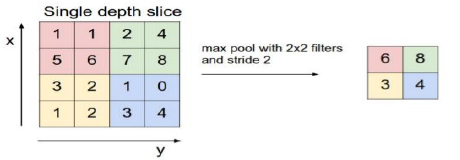
\includegraphics[width=0.8\linewidth]{imgs/chapter11/img12}
			\caption{Max-pooling}
			\label{fig:chapter11-12}		
		\end{minipage}%
		\begin{minipage}{.5\textwidth}
			\centering
			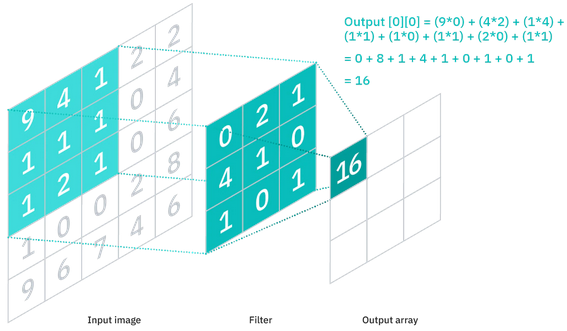
\includegraphics[width=0.8\linewidth]{imgs/chapter11/img18}
			\caption{Convolutional layer}
			\label{fig:chapter11-18}
		\end{minipage}
	\end{figure}

		\subsubsection{Convolutional layers}
		I convolutional layers \ref{fig:chapter11-18} sono il nucleo di una CNN, consistono di un insieme di filtri, ognuno dei quali copre una piccola porzione spaziale dei dati di input o campo recettivo.
		Ogni filtro viene convoluto attraverso la dimensione dei dati di input, producendo una mappa di feature multidimensionale.
		La rete \textbf{impara} i filtri che si attivano quando trovano uno specifico tipo di feature a una certa posizione spaziale nell'input. 
		In una CNN ci sono tre tipi di layer: convoluzionali, pooling e fully connected. 
		Tipicamente si comincia da un layer convoluzionale, che \`e seguito da uno di max-pooling, poi un'altro convoluzionale, un'altro di max-pooling, ..., i layer finali sono sempre fully-connected.
		
		\subsubsection{Non linearity}
		La non linearity aumenta la non linearity dell'intera architettura senza avere effetto sui campi recettivi del livello di convolution.
		$$y_{i,j} = f(a_{i.l})$$
		Per esempio $f(a) = [a]_+$ o $f(a) = sigmoid(a)$.
		
		\subsubsection{Pooling}
		Il pooling riduce la dimensione spaziale della rappresentazione riducendo la quantit\`a di parametri e la computazione della rete, controllando l'overffitting.
		$$x_{i,j} = \max\limits_{|k|<\tau, |l|<\tau}y_i - k_{ij} - l$$
		Inoltre fornisce invarianza rispetto alle traslazioni.
		
		\subsubsection{Esempi di architetture}
		\begin{multicols}{2}
			\begin{itemize}
				\item LeNet.
				\item AlexNet.
				\item VGG.
				\item GoogleNet.
				\item ResNet.
			\end{itemize}
		\end{multicols}

	\subsection{Conclusione}
	Le CNN a differenza delle feedforward vanilla presentano un ordinamento spaziale: ad ogni layer le unit\`a sono organizzate in griglie a $2D$, le feature maps.
	Ognuna di esse \`e il risultato di una convoluzione.
	Lo stesso filtro convoluzionale \`e applicato ad ogni locazione.
	I pesi sono diversi attraverso le feature maps.
	Una unit\`a a una particolare locazione sulla griglia pu\`o solo ricevere l'input da unit\`a a una locazione simile al livello inferiore.
	Si necessita di dati con labels ed \`e flessibile a molte applicazioni.

\section{Altre reti neurali}
Esistono diversi modelli di reti neurali per diverse necessit\`a.
In particolare fino ad ora si \`e discusso su problemi di predizione in cui si hanno input e output di dimensione fissa.
Ci sono casi di sequential prediction tasks in cui l'input o l'output sono sequenze di lunghezza variabile.
Si usano per esempio nella predizione dei frame video. 
Questi si risolvono attraverso recurrent neural networks.

	\subsection{Recurrent neural networks}
	Nelle recurrent networks input precedenti vengono utilizzati per influenzare le decisioni su input successivi.
	Questo si ottiene attraverso dei layer ricorsivi, in cui la rappresentazione nascosta al tempo $t$:
	$$h_t = f_w(x_t, h_{t-1})$$
	Si nota come la funzione di $W$ dipende sia dall'input $t$ che dallo stato precedente. 
	Per una rappresentazione grafica osserva la figura \ref{fig:chapter11-13}.
	
	\begin{figure}
		\centering
		\begin{minipage}{.5\textwidth}
			\centering
			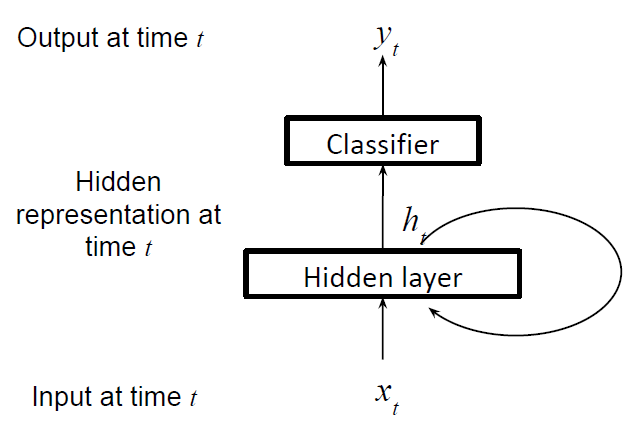
\includegraphics[width=0.8\linewidth]{imgs/chapter11/img13}
			\caption{Recurrent neural networks}
			\label{fig:chapter11-13}			
		\end{minipage}%
		\begin{minipage}{.5\textwidth}
			\centering
			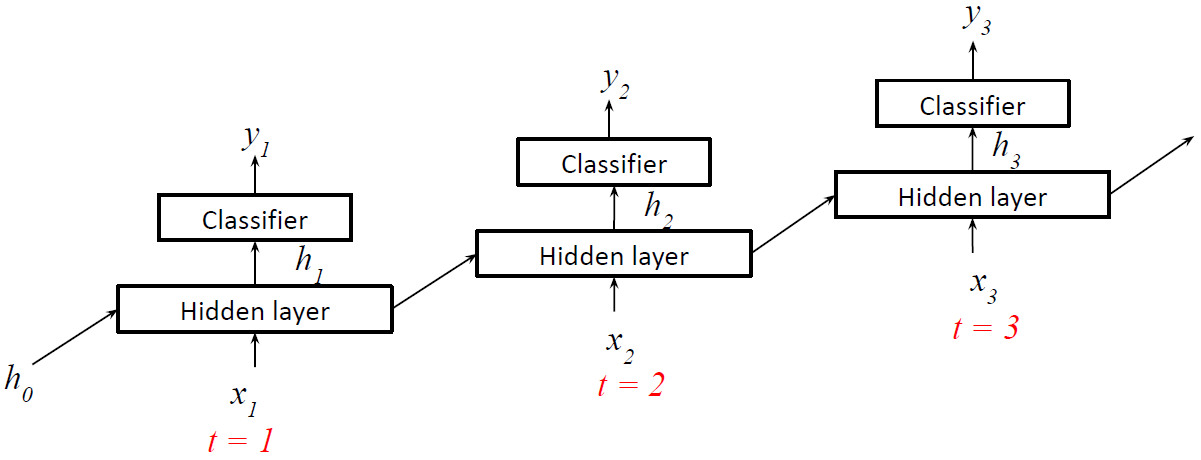
\includegraphics[width=1\linewidth]{imgs/chapter11/img17}
			\caption{Visualizzazione alternativa recurrent neural networks}
			\label{fig:chapter11-17}
		\end{minipage}
	\end{figure}
	
	
	In particolare si nota come considerando una visione ``svolta'' dei layer ricorsivi si possono mappare diversi input a diversi output in relazione:
	\begin{multicols}{2}
		\begin{itemize}
			\item One-to-one.
			\item One-to-many
			\item Many-to-one.
			\item Many-to-many.
		\end{itemize}
	\end{multicols}
	
	Le RNN hanno applicazioni per esempio nel campo del language processing in cui si chiede al modello di generare del testo.
	
	\subsection{Autoencoders}
	Gli autoencoders sono un esempio di unsupervised learning.
	Sono simili a feedforward neural networks.
	Il loro scopo \`e quello di comprimere automaticamente dell'informazione.
	Hanno una forma a clessidra in cui i layer in mezzo sono quelli pi\`u piccoli (chokepoint della rete).
	Tutto quello che si trova fino alla met\`a \`e l'encoder, quello dopo il decoder.
	La rete si addestra attraverso backpropagation e l'errore \`e la differenza tra l'output e l'input.
	Possono essere costruiti simmetricamente anche rispetto ai pesi.
	Lo scopo \`e pertanto impara una rappresentazione a meno dimensioni del training data.
	L'encoder \`e passato da essere un linear + nonlinearity come sigmoid, a un deep, fully connected a ReLu con CNN.
	$z$ nel mezzo \`e pi\`u piccolo di $x$: si svolge una dimensionality reduction \ref{fig:chapter11-15}.
	Le feature dovrebbero catturare fattori significativi di variazioni nel dato.
	Un esempio per capire la differenza tra output e input \`e la L2 loss function $||x-\hat{x}||^2$.
	Dopo il training si scarta il decoder e l'encoder pu\`o essere utilizzato per inizializzare un modello supervised che permette un fine-tuning insieme al classificatore. 
	Quest'ultimo avr\`a prestazioni migliori in quanto andr\`a ad operare su dati di minore dimensione \ref{fig:chapter11-16}. 
	
	\begin{figure}
		\centering
		\begin{minipage}{.5\textwidth}
			\centering
			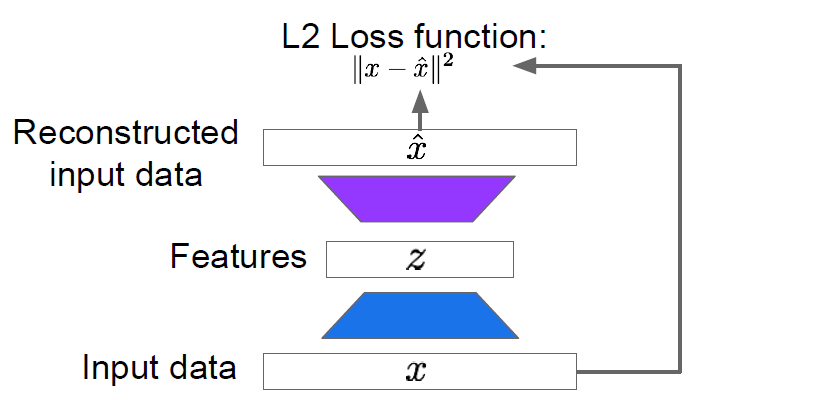
\includegraphics[width=1\linewidth]{imgs/chapter11/img15}
			\caption{Autoencoders}
			\label{fig:chapter11-15}
		\end{minipage}%
		\begin{minipage}{.5\textwidth}
			\centering
			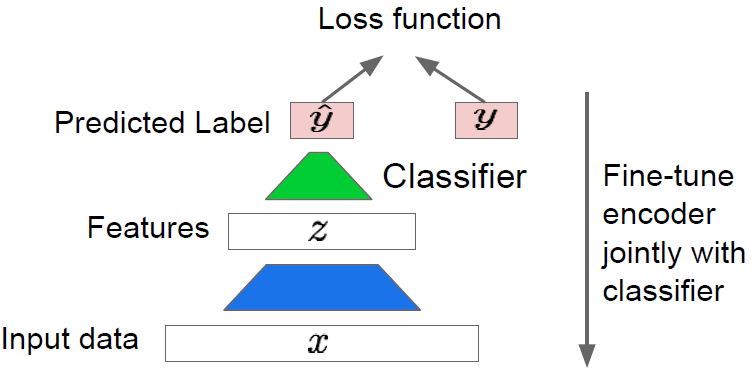
\includegraphics[width=1\linewidth]{imgs/chapter11/img16}
			\caption{Autoencoder per l'inizializzazione di un modello supervised}
			\label{fig:chapter11-16}
		\end{minipage}
	\end{figure}